\documentclass[12pt,
border=1pt]{standalone}
\usepackage{pgfplots}
\usepackage{amsmath}
\usepackage{amssymb}

\pgfplotsset{compat=newest,
	width=6cm, height=5cm,
	xtick pos=left, ytick pos=left,
	%            scaled x ticks=real:1e-6,
}
% Kernel 2 FP64
\begin{document}
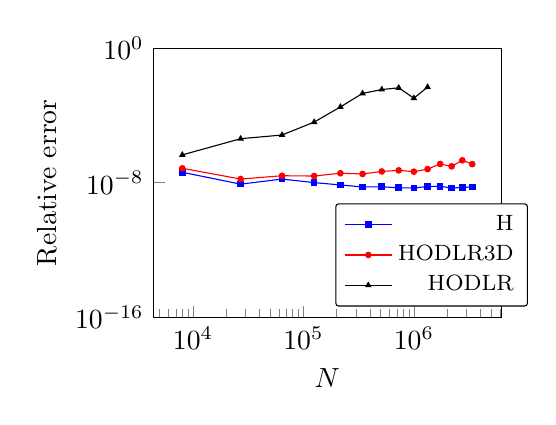
\begin{tikzpicture}[every mark/.append style={mark size=1pt}]
	\begin{axis}[xlabel={$N$},
	ylabel={Relative error},
%		legend pos=south east,
		legend style={
                at={(0.8,0.04)},
               anchor=south,
               legend columns=1,
               cells={anchor=east},
              font=\footnotesize,
               rounded corners=1pt,
               },
		xmode = log,
	    ymode = log,
	   % xmin = 1e3,
	   % xmax = 1e6,
	    ymin = 1e-16,
	    ymax = 1e-0,
	   % xtick={1e-10, 1e-8, 1e-6,  1e-4,  1e-2},
	   % ytick={1e-8, 1e-6,  1e-4,  1e-2, 1e-0}
		]
% 		\addplot[
% 		color=red,
% 		mark=o,
% 		] coordinates {

% (13824,2.031870e-07)
% (110592,1.264230e-07)
% (884736,1.085520e-07)
% (7077888,1.004550e-07)
% 		};
		\addplot[
		color=blue,
		mark=square*,
		] coordinates {
(8000,4.190530e-08)
(27000,8.260650e-09)
(64000,1.650610e-08)
(125000,1.020340e-08)
(216000,7.377760e-09)
(343000,5.629230e-09)
(512000,5.752400e-09)
(729000,5.012510e-09)
(1000000,4.911500e-09)
(1331000,5.951520e-09)
(1728000,6.160010e-09)
(2197000,4.853100e-09)
(2744000,5.274050e-09)
(3375000,5.585000e-09)
% (4096000,3.566110e-09)
% (4913000,4.716700e-09)
% (5832000,4.023940e-09)
% (6859000,7.316710e-09)
		};
		\addplot[
		color=red,
		mark=*,
		] coordinates {
(8000,7.227830e-08)
(27000,1.658720e-08)
(64000,2.605630e-08)
(125000,2.512710e-08)
(216000,3.665400e-08)
(343000,3.330930e-08)
(512000,4.694020e-08)
(729000,5.451460e-08)
(1000000,4.561370e-08)
(1331000,6.466630e-08)
(1728000,1.304910e-07)
(2197000,9.467980e-08)
(2744000,2.163560e-07)
(3375000,1.280640e-07)
		};
		
		\addplot[
		color=black,
		mark=triangle*,
		] coordinates {
(8000,4.531300e-07)
(27000,4.149330e-06)
(64000,6.874090e-06)
(125000,4.021570e-05)
(216000,3.210050e-04)
(343000,2.048430e-03)
(512000,3.470940e-03)
(729000,4.395700e-03)
(1000000,1.063030e-03)
(1331000,4.853190e-03)
		};		
		\legend{H, HODLR3D, HODLR}
	\end{axis}
\end{tikzpicture}
\end{document}